\documentclass{article}
\usepackage{graphicx} % Required for inserting images
\usepackage{amsmath}
\usepackage{cleveref}
\usepackage{todonotes}

\newcommand{\argmax}{\operatorname{argmax}}

\title{Ode to KL}
\author{Tomáš Gavenčiak, Václav Rozhoň}
\date{February 2025}

\begin{document}

\maketitle

\tldrbox{
This text explains the formula for KL divergence: $D(p,q) = \sum p_i \log p_i/q_i$. It also explains all kinds of applications that this formula has. 
}

This text introduces and explains the so-called KL divergence, sometimes also known as relative entropy. It is a function that takes two distributions as input—one being the ``true'' distribution and the other our model for it—and outputs a measure of how well the model fits the true distribution.

Surprisingly, understanding this function explains many concepts in probability, statistics, machine learning, and deep learning. This text came about when the two authors were chatting about their favorite topics in probability, as well as some arcane technical problems in probabilistic modelling they had been pondering. They realized that there are some aspects (or takes) on probability theory that are not typically covered in standard university courses (but only after spending way too much time chatting with people, procrastinating on the internet, reading obscure LessWrong blog posts, and finding hidden gems in long technical books). This text aims to fill a small gap by focusing on KL divergence and its applications.

\section{A Few Riddles}

\subsection{Polling}

The next US elections are coming and you want to estimate which of the two parties is going to win the popular vote. Here's how: You will sample a few random US citizens and ask them who they vote for, the estimate you compute from this sample is hopefully a good approximation of reality. If we assume a simplified model where every citizen votes for one party, they are truthful, and won't change their opinions in the future\footnote{Of course, those assumptions are very unrealistic but bear with us. }, you can compute that asking 1000 people is enough to get an estimate that is probably\footnote{To be precise, with probability ?? \%} within one per cent of the right answer. I think this is astonishing! Think of it, regardless of how many people live in the country, 1000 random citizens are enough to get the answer within one per cent. 

But also, in reality, all us elections are incredibly close; we already know that both Democratic and Republicans are going to get around 50\%. So we should perhaps get a bit bigger sample sufficient to get an estimate that is likely to be correct within $0.1\%$. The question is, how many people should we sample this time? 

1) about 3000
2) about 10000
3) about 100000

The correct answer is about 100000. In fact, if we want to be close up to an error of $\eps$, we need about $1/\eps^2$ samples. This means that getting better estimates is getting much more expensive! This is one of the reasons why most polling estimates do not bother asking more than about 1000 people -- even in the most idealistic scenarios, you have to ask 4 times more people to get twice as good estimate. 

The question is: why $1/\eps^2$? 

\subsection{Financial Mathematics}

The following data shows how the price of Bitcoin and the S\&P index changed each day over the last year. As you might have guessed, the average change is slightly positive, but there is also large variance. For example, the average daily S\&P change is about \$0.5, but the standard deviation is \$3, meaning that a typical daily change is between approximately -\$2.5 and +\$3.5 per share.

Question is

But how should we model the changes in more detail? One way is using the so-called normal distribution with shape \(e^{-x^2}\); another possibility is the Laplace distribution, with shape \(e^{-|x|}\).

Eyeballing the data, it seems that the normal distribution is a better fit for the S\&P index, while the Laplace distribution is a better fit for Bitcoin. KL divergence can measure how well a true distribution (the histogram from last year) is fitted by a model (normal or Laplace). It is zero if the two distributions are identical, and the more different they are, the larger the divergence. You can see in the legend that KL agrees that Laplace is a better fit for Bitcoin and normal is a better fit for the S\&P.

\begin{figure}
    \centering
    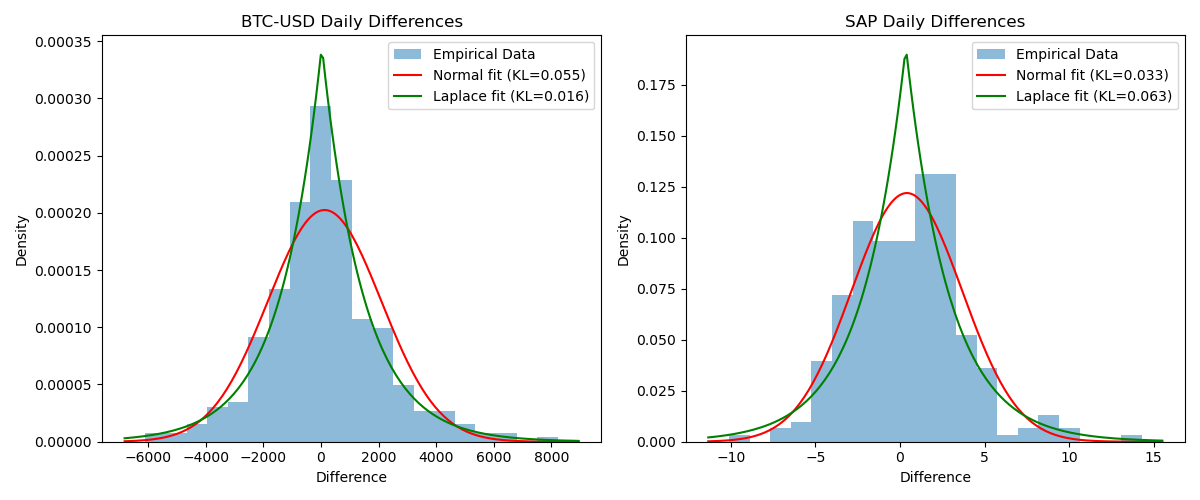
\includegraphics[width=0.9\linewidth]{fig/financial.png}
    \caption{Caption}
    \label{fig:enter-label}
\end{figure}\todo{for five-year data Laplace is better even for S\&P because of outliers, I guess}

But... do we have a story explaining why this is? And why did we even try the normal and Laplace distributions as potential fits rather than some other distributions?

\subsection{Statistics}

In the old days (and in some countries even today), people measured lengths in feet. But how do you determine the length of a foot? You could measure the foot of the local warlord, but then you would have to change it once the warlord is replaced.

It's a bit better to ask 16 random people (as in \cref{fig:rod}) and compute their mean foot length as
\[
\bar X = \frac{1}{16} (X_1 + \dots + X_{16}),
\]
which will be a fairly stable estimate that will hopefully remain similar the next time you perform this experiment.

\begin{figure}
    \centering
    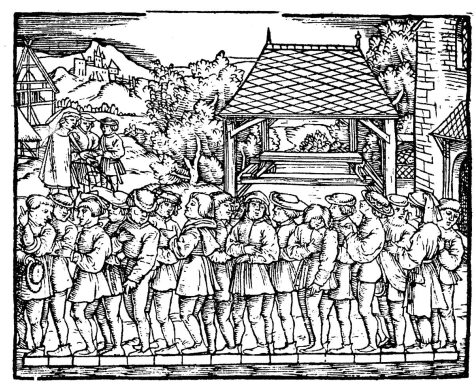
\includegraphics[width=0.9\linewidth]{fig/rod.png}
    \caption{Determining the length of the foot in 1522.}
    \label{fig:rod}
\end{figure}

How good is this estimate? Typically, one would gauge it by estimating the standard deviation using the formula
\[
\bar \sigma^2 = \frac{1}{16} \sum_{i=1}^{16} (X_i - \bar X)^2.
\]
But is this formula correct? Should we divide by 15 instead? Or maybe 17?

Click on the right answer: 

The issue with choosing the right coefficient is not that one of the options (dividing by \(n-1\), \(n\), or \(n+1\)) is uniquely correct—they are all defensible in (frequentist) statistics.

The coefficient \(1/(n-1)\) corresponds to the so-called unbiased estimate, \(1/n\) gives the maximum likelihood estimate, and \(1/(n+1)\) minimizes the mean squared error.

\subsection{Predictions}

It would be great to know what the future holds—or at least to know someone who does. To this end, you have gathered a bunch of experts and asked them to assign probabilities to a list of events for the coming year. Each expert provides an estimate for each event.

When the year ends, you know for each event whether it occurred or not. The question is, how do we score the experts so that we can pick the best ones? For example, which of the experts would you think is the best one in this case? 

\todo{add simple example table}

\subsection{Information Theory}

Suppose you are interested in two things. First, whether a day is rainy or sunny—say, with probabilities 30\% and 70\%, respectively. Second, how you commute to work (e.g., walk, bike, or take the bus with probabilities 20\%, 30\%, and 50\% respectively).

Knowing these two marginal distributions does not give you the full picture. You can form a 2$\times$3 table representing the joint distribution of these outcomes.

If the two distributions were independent, the probability in each cell would be the product of the marginal probabilities. For example, modeling the distributions as independent, we would guess that the probability of rain and walking is \(0.3\times0.2=0.06\) (i.e., 6\%). But in fact, it is much lower (since I don't want to walk in the rain).

The question is: Is there a good measure of how far the joint distribution is from being independent? For example, given two tables, how would you determine which one is closer to independence?

As a potential, though not entirely satisfactory, answer, if the two variables were numerical, we might use correlation. Correlation is 0 if the variables are independent and 1 if they are perfectly correlated. (For example, in people, height and weight might correlate with 0.??.) But this approach does not work in our example since we can't assign numbers to categories like walk/bike/bus. Also, two variables can be far from independent yet have zero correlation (e.g., ...). Can we intuitively understand when does using correlation make sense and when it does not? 

\subsection{Deep learning}

Think of a large language model (LLM) like GPT4. This model is given some text, does some computation, and outputs the next token\footnote{Token is just a small group of letters, so feel free to think that it outputs the next letter or syllable or word. } in the text. In fact, it always outputs a distribution $p$ over all of the possible tokens (usually there are about ?? of them). This is why it's simple to make the LLMs output different answers on the same text. 

Your task is to train a new, smaller model that's as good as the base GPT4 model. You have already prepared a lot of texts on the internet. For each text, you will first run GPT4 to output its distribution $p$ over then next token. Then, you run your small model to obtain a different distribution $q$. You would like to make sure that $q$ is as close to $p$ as possible, but to do so, we first have to come up with a good function $f(p,q)$ that can tell us how far $p$ and $q$ are. So, what would be a good choice of this function $f$? 


\subsection{Machine Learning}

Have you noticed that certain functions appear frequently in machine learning?

For example, consider \(x^2\): The most basic clustering algorithm, \(k\)-means, minimizes the sum of squared distances, and the same holds for linear regression. Why use \(x^2\)? Why would it mean to use \(|x|\) or \(x^4\) instead?

Or consider the logarithmic function. Standard machine learning tools like logistic regression involve logarithms, and neural nets are often optimized using the so-called cross-entropy loss—which takes logarithms of probabilities. %Also, when training neural nets to output probabilities, we typically work with logits (logarithms of probabilities). Why?
Some formulas in machine learning are true beasts. Consider e.g. the loss function for the so-called logistic regression:


And then there are beasts like variational autoencoders (The architecture behind DALLE and Midjourney, at least until 2025) that are trained using this beastly loss function:

Where are these horrific expressions getting from? What's their meaning?



\subsection{Modelling}

\todo{je lepsi pohadka? nevim proc bych modeloval zrovna restauraci. treba vybirani auta mi prijde jako vic sexy priklad, ale tam zase ruzna auta maji treba ruznou reklamu...}

A customer comes to a restaurant. Each meal on the menu has a specific tastiness value, which we conveniently assume is known. If the customer spends enough time considering all the meals, she will pick the one with the highest tastiness. But if she is extremely hungry, she might simply choose a random meal. The question is: How should we model the situation in between—when the customer spends some time looking at the menu but not enough to always pick the tastiest item?

More mathematically speaking, given \(n\) numbers \(a_1, \dots, a_n\), can we find a parameter \(\lambda\) and a natural family of probability distributions such that \(\lambda=0\) corresponds to the uniform distribution and \(\lambda=+\infty\) corresponds to picking the maximum value (i.e., \(\argmax_{i} a_i\))?

You sometimes encounter this type of question when constructing a probabilistic model. There are many degrees of freedom in constructing a probability distribution, so how do we pick the ``most natural'' one that interpolates between complete order and total randomness?

This quandary is typically resolved by what's known as the maximum entropy principle. In this case, the principle dictates that we should choose the so-called softmax distribution. How does this principle work, and where does it come from?

Here's the example of the softmax distributions. There is one parameter, $\lambda$, and as you change it, you interpolate between taking the maximum, and sampling from uniform distributions (the parameter $1/\lambda$ is often called temperature). 


\subsection{Random pi program}

Here's a riddle. Consider the set of all C programs of length 1000 characters (i.e., the file has 1000 bytes if saved in ASCII) that print the first million digits of $\pi$. Let's sample one such program uniformly at random. How is it going to look like? 

\subsection{Algorithm design}


how to choose the best expert? 
How do you find Nash equilibrium in two person games?

\subsection{Logistics}

-- You can skip a lot of stuff

\section{Definition of KL divergence}

\tldrbox{
KL divergence measures how well a ``true distribution'' or empirical data $p$ is fitted by a model distribution $q$. The formula is $D(p|q) = \sum p_i \log p_i / q_i$. 

    The meaning behind this formula is that if you keep sampling from the true distribution $p$ and applying Bayes theorem, KL tells you how quickly you are able to distinguish whether you are sampling from $p$ or $q$. 
}

KL divergence is a measure that takes two distributions as input: the true distribution \(p\) (represented by \(p_1, \dots, p_n\)) and the model distribution \(q\) (represented by \(q_1, \dots, q_n\)), with both summing to one.

KL divergence is defined as
\begin{align}
    \label{eq:kl_definition}
    KL(p, q) = \sum_{i = 1}^n p_i \log \frac{p_i}{q_i}.
\end{align}
What is the intuition behind it?

First, here is a simple widget where you can change the probabilities of \(p\) and \(q\) and see what the KL divergence is.

Notice that there is a certain asymmetry between \(p\) and \(q\). If you push the value \(q_i\) to zero for some \(i\) where \(p_i > 0\), the KL divergence becomes infinite. This reflects the fact that if your model predicts an event is impossible and it occurs, your model is infinitely bad. On the other hand, if \(p_i=0\) and \(q_i>0\), nothing dramatic happens—being prepared for an event that never occurs only slightly detracts from your performance.

Sometimes, KL divergence is introduced as ``something like a distance,'' but unfortunately it is not symmetric, so it is not a true distance metric. In fact, the asymmetry is important because the two distributions play different roles: \(p\) is the true distribution, and \(q\) is our model for it.

We now discuss two mathematical intuitions for the formula.

\subsection{Expected Distinguishing Evidence}

First, a quick recap of Bayes' theorem.

Suppose you have a coin and you consider two hypotheses:
\begin{enumerate}
    \item The coin is biased: it shows heads with probability 0.4 and tails with probability 0.6.
    \item The coin is fair: it shows heads with probability 0.5 and tails with probability 0.5.
\end{enumerate}
Assume that the coin is actually biased (i.e., hypothesis 1 is true). However, initially you believe the coin is probably fair, assigning probabilities \(2/3\) to it being fair and \(1/3\) to it being biased (or odds \(1:2\) for biased to fair).

\todo{let's add some footnote that derives it}
Now, note that under hypothesis 1 (biased), the probability of heads is 0.4, while under hypothesis 2 (fair) it is 0.5. The ratio of these probabilities is \(0.4:0.5\), or equivalently \(4:5\). Bayes' theorem tells us to update your odds by multiplying the prior odds by this likelihood ratio:
\[
1:2 \quad \times \quad 4:5 \quad = \quad 4:10 \quad = \quad 2:5.
\]
This corresponds to a posterior probability of about 29\% that the coin is biased.

You can gather more evidence by flipping the coin a few more times. Suppose you flip the coin twice more and get more tails. Using Bayes' theorem, you multiply the likelihood ratios for each flip:
\[
1:2,\quad 40:50,\quad 60:50,\quad 60:50 \quad \Longrightarrow \quad 144:250,
\]
which corresponds to about a 37\% probability that the coin is biased.

How quickly are we gathering evidence in favor of the coin being biased? To analyze this, it is simpler to take logarithms of the ratios so that we add rather than multiply. Instead of multiplying by the ratio \(40/50\), we add \(\log_2(40/50) \approx -0.32\) and for \(60/50\) we add \(\log_2(60/50) \approx 0.26\).

Since \(\log_2(1/2) = -1\), we can describe our three-flip experiment as follows: We started with \(-1\) bit of prior evidence favoring the coin being biased. After the first flip, the evidence becomes \(-1-0.32 = -1.32\) bits; after the second flip, \(-1.32+0.26 = -1.06\) bits; and after the third, \(-1.06+0.26 = -0.8\) bits.

In general, since the coin is biased, each flip yields \(0.26\) bits of evidence with probability 0.6 and \(-0.32\) bits with probability 0.4. The average evidence per flip is
\[
0.6\cdot 0.26 - 0.4\cdot 0.32 \approx 0.03\text{ bits}.
\]
Notice that this expression is exactly the KL divergence in \cref{eq:kl_definition} computed for the true distribution \((0.6,0.4)\) and the model \((0.5,0.5)\).

The positive average evidence indicates that, on average, each flip provides approximately 0.03 bits of evidence in favor of the true (biased) hypothesis. By the law of large numbers, if you flip the coin \(n\) times, you would expect to accumulate about \(0.03\cdot n\) bits of evidence.

[example where we sample 10 times]

Compute one column. We can also write the expected value of this like this. This is called cross entropy. 
... this is called entropy, relative entropy. \footnote{It breaks my heart to use the term KL divergence combining two random letters with a term that's too technical to properly explain even in this text. Especially when relative entropy is so self-explanatory. However, the KL name is pretty much settled these days in the machine learning community. }


\paragraph{Zooming Out}  
Zooming out, we can view KL divergence as the expected evidence obtained per flip in favor of the true hypothesis \(p\) when comparing it against an incorrect model \(q\). Here, \(p_i\) in \cref{eq:kl_definition} represents the probability of the \(i\)th outcome under the true distribution, and the term \(\log(p_i/q_i)\) represents the evidence for the true hypothesis when outcome \(i\) occurs. The overall KL divergence is the expected evidence per trial, with the logarithm ensuring that evidence accumulates additively.

KL divergence is thus about the evidence, not the prior. This is why it is relevant in both classical (frequentist) and Bayesian statistics.

\subsection{Natural Measure}


\todo{add discussion that KL is aditive for independent distributions}
Here is another thought experiment leading to KL divergence. Suppose we want to find a reasonable function \(f(p,q)\) that measures how well the true distribution \(p\) is approximated by a model distribution \(q\).

Instead of proposing concrete formulas immediately, we can ask what properties such a function should satisfy. Consider joint distributions—say, the joint distribution over weather (sunny/rainy) and commuting methods (walk/bike/bus) from a previous example.

Such a distribution can be represented as a table with six numbers (which we can input into \(f\)), or equivalently using conditional probabilities as a ``decision tree'' where you first learn whether it rains and then, given that, decide on walking, biking, or taking the bus.

On the left is a picture of the true distribution, and on the right is our model. Suppose the second model differs in the probabilities for sunny/rain but has the same conditional probabilities for walk/bike/bus given the weather as reality. In this case, I would argue that \(f\) should depend only on the difference in the weather probabilities. That is, we require that
\[
f(\text{table1}, \text{table2}) = f((0.4, 0.6), (0.5, 0.5)).
\]
\todo{let's do this or maybe just the "chain rule" and explain using some kind of story where we take microscope}
On the other hand, consider a situation where our model for weather is spot on and our model for commuting in sunny conditions is perfect—but in the rain case, it is a bit off. In this case, the function \(f\) applied to the full tables should equal \(f\) applied to the commuting distributions for the rainy case, weighted by the true probability of rain. For instance,
\[
f(\text{table1}, \text{table2}) = 0.3\cdot f\bigl((\cdot), (\cdot)\bigr).
\]

Generalizing these thought experiments, it seems natural to require that if we can decompose two distributions \(p\) and \(q\) as joint distributions \((p_1,p_2)\) and \((q_1,q_2)\), then
\[
f((p_1, p_2), (q_1, q_2)) = f(p_1, q_1) + \sum_i p_i\cdot f\Bigl(p_2(\cdot|i), q_2(\cdot|i)\Bigr).
\]
\todo{notation clarification}

A priori, it is not clear whether any function \(f\) satisfies this property, since there are many ways to represent a joint distribution using different trees. Remarkably, this constraint almost uniquely characterizes KL divergence.

\begin{theorem}
    Let \(f\) be a function on pairs of probability distributions on an \(n\)-element set. Suppose \(f\) satisfies the following constraints:
    \begin{enumerate}
        \item 
        \[
        f((p_1, p_2), (q_1, q_2)) = f(p_1, q_1) + \sum_i p_i\cdot f\Bigl(p_2(\cdot|i), q_2(\cdot|i)\Bigr),
        \]
        \item \(f(p,q)\) is nonnegative, with \(f(p,q)=0\) if and only if \(p=q\).
        \item \(f(p,q)\) is continuous. \todo{check if that's all}
    \end{enumerate}
    Then,
    \[
    f(p,q) = c\, KL(p,q)
    \]
    for some positive constant \(c\), and conversely.
\end{theorem}

For example, we require nonnegativity because working with \(f(p,q) = -KL(p,q)\) would be counterintuitive. Continuity is required for technical reasons related to Vitali's paradox. Note that \(f\) is defined only up to a constant factor, which is equivalent to the choice of logarithm base in the definition of \(KL\). We use base 2 because we are computer scientists and like to think in bits (physicists might choose \(\mathrm{e}\)); it doesn't really matter.

\paragraph{Nonnegativity}



\subsection{Proving the Easy Direction}

We will not prove that KL divergence is the only function satisfying the above constraints, but we will at least verify that it does satisfy them:
\begin{enumerate}
    \item Write it down.
    \item See, for example, \href{https://stats.stackexchange.com/questions/335197/why-kl-divergence-is-non-negative}{this discussion} for a proof of nonnegativity.
    \item We will not delve into the technical details of continuity, but suffice it to say that KL divergence is continuous.
\end{enumerate}

\subsection{Application: training smaller models }

Let's solve one of our riddles. 

You may not be surprised to learn that for this task, people are usually optimizing the KL divergence $D(p,q)$ between the two distributions. 

What about other options, like minimizing the $\ell_1$ norm, i.e., $\sum |p_i - q_i|$? or $\ell_2$ norm, i.e., $\sum (p_i - q_i)^2$? Doing that would perhaps also work reasonably well, but there is something very uneasy about those approaches. What's the bigger problem out of these two? 
1. $p_i = 0.5, q_i = 0.49$
2. $p_i = 0.01, q_i = 0.0$
The standard geometrical norms ($\ell_1, \ell_2$) treat both of these situations as the same failure. KL, though, understands that while in the first situation, the difference is pretty negligible, in the second situation, the model failed utterly and miserably!


\subsection{Application: Distance from Independence}

We can now solve one of the earlier riddles: Given a joint distribution $r = (p,q)$, how far is it from being independent? 

Let's try to fit the problem into using KL divergence. We want the answer to be KL between two distributions, one of them ``the true one'', the other ``a model for it''. 

So, what should be the ``true distribution''? Here it's pretty natural, we have the true joint distribution $r$ between $p$ and $q$. Next, what should the model be? Since we are trying to measure the ``distance from independence'', let's choose the model the joint distribution \emph{as if $p$ and $q$ were independent}. That is, let's choose the distribution $s = p \times q$ which is the product distribution between $p$ and $q$. 

\[
I(p;q) = KL\bigl((p,q), (p\times q)\bigr).
\]
This measure is known as the mutual information. It's one of those formulas that pop up at all kinds of places, especially in information and coding theory. For example, when you analyze the problem of sending some data over a wire that can flip each sent bit with some probability, the mutual information between the original data on one end of the wire and the noisy data on the other end of the wire is a key quantity to understanding how much the unreliability of the wire slows down the transmission. Mutual information is also used in practice to assess how far variables are from being independent, especially when correlation is not applicable (e.g., when the data are categorical).

% \paragraph{More on correlation vs mutual information}


% Here's also one, a bit more theoretical, application of mutual information. I've already mentioned the correlation. To remind you, if you have two random variables $X,Y$, you can compute their correlation as 
% \[
% corr(X,Y) = \frac{E[(X-E[X])(Y-E[Y]]}{\sqrt{E[(X-E[X])^2]E[(Y-E[Y])^2]}}
% \]

% Intuitively, correlation is measure the linear dependence, high correlation means that if you plot the distribution in 2D plane and fit the best line using linear regression, the line is a good fit for the data. 

% On the other hand, mutual information measures in the full generality what's the best fit for the data. It does not have to be a line, could be a parabola or not even a curve. 

% There are some simple cases where both measures ``agree''. For example, consider the case of the so-called joint Gaussian distribution $(X,Y)$ where $Y = \alpha X + \beta + N(0, \sigma^2)$. That is, to sample from this distribution, we first sample $X$ from a gaussian distribution, and then to get $Y$, we multiply $X$ by some number $\alpha$, add $\beta$, and finally add small additional gaussian noise. It turns out that in this case there's a simple formula relating the correlation $corr(X,Y)$ and mutual information $I(X,Y)$:
% \[
% I(X,Y) = -\frac12\ln(1-corr(X,Y)^2)
% \]
% The exact formula is not so important, the important part is how knowing one of them means you also know the other one (except that if you know $I(X,Y)$, you don't know what $corr$ is, only what $|corr|$ is). The way I look at it is that if you are modelling data as coming from Gaussian distribution (which is quite common, by the way), you ``can't beat the line''. That is, if you want to predict $Y$ from $X$, you can't really beat the approach of fitting the best line (or plane) by linear regression. 

% On the other hand, if your data was not generated by this incredibly nice and idealized process, you can typically ``beat the line'' and mutual information tells you the limit for how much you can beat it. 

\section{Entropy, Cross-Entropy, and Relative Entropy}

\tldrbox{
You can split the formula for KL divergence as a difference between cross entropy $H(p,q)$ and entropy $H(p)$. 

Cross entropy between distributions $p$ and $q$ is measuring how surprised you are when you keep sampling from $p$ and using $q$ as your model of the data. If $p = q$, it's called entropy. 
}

It is sometimes helpful to rewrite the formula for KL divergence as a difference of two expressions:
\begin{align}
\label{eq:split_KL}
\sum_i p_i \log \frac{p_i}{q_i} 
= \sum_i p_i \log \frac{1}{q_i} 
- \sum_i p_i \log \frac{1}{p_i},
\end{align}
where we used the identity \(\log p_i = -\log(1/p_i)\).

The left-hand side is the KL divergence (also called relative entropy). The term \(\sum_i p_i \log \frac{1}{q_i}\) is called the cross-entropy, and \(\sum_i p_i \log \frac{1}{p_i}\) is the entropy.

How do we interpret this equation? One way is to return to our initial example of coin flips.

\begin{center}
[picture]
\end{center}

Imagine a balance sheet with two columns: the left column lists the surprise (in bits) based on the true distribution \(p\), and the right column lists the surprise based on the model \(q\). For instance, if the model assigns a probability of 1\% to heads, then whenever heads occurs the surprise is \(\log(1/0.01) \approx 6.6\) bits—a significant surprise!

The KL divergence is the difference between these two surprises. Alternatively, we can consider the surprises separately. The first column, which gives the average surprise when data are generated by \(p\) and modeled by \(p\), is the entropy of \(p\). It quantifies the inherent uncertainty in the distribution. For example, if \(p\) is degenerate (100\% heads), the surprise is \(\log(1)=0\). In contrast, for a uniform distribution over 16 outcomes, each outcome gives 4 bits of surprise.

The second column represents the average surprise when data are generated by \(p\) but modeled by \(q\), which is the cross-entropy.

\paragraph{Additivity}
Just like KL, the crossentropy and entropy are additive for independent distributions

\subsection{Application: Predictions}

As the next application of KL / crossentropy, let's solve prediction. Let us now consider an application of \cref{eq:split_KL}. Recall the riddle about grading experts who predict future events.

\todo{add simple example table}

In this case, we include an extra row in the table for the ``true'' probabilities (whatever that means\footnote{I feel a bit uneasy discussing this row since I view probability as subjective; I am not sure what an objective probability for, say, the next US president means.}). 

To grade an expert's predictions, let \(p\) denote the true probabilities of events and \(q\) denote the expert's predicted probabilities. We define the expert's score as
\[
KL(p,q).
\]
For example, if an expert's predictions are 30\% and 40\%, then \(q\) is represented as the product distribution of \((0.3,0.7)\) and \((0.4,0.6)\). That is, we think of the expert's prediction as two distributions rather than two numbers. In this case, the formula for \(KL(p,q)\) can be written as
\[
KL(p,q) = \sum_i \left[p_i\log\frac{p_i}{q_i} + (1-p_i)\log\frac{1-p_i}{1-q_i}\right].
\]

However, there is a problem with this formulation—in reality, we do not know \(p\)! Instead, we can set up a grading scheme such that, in the long run, the expert's average score converges to the cross-entropy. Specifically, we charge the expert \(\log(1/q_i)\) whenever an event occurs and \(\log(1/(1-q_i))\) whenever it does not. This scoring rule, known as the log score, yields an expected score of
\[
\sum_i \left[p_i\log\frac{1}{q_i} + (1-p_i)\log\frac{1}{1-q_i}\right],
\]
which is exactly the cross-entropy between the true distribution and the expert's model.

Note that we can only ensure correct grading in the long run. For instance, if you ask an expert about a single event—say, whether a random card from a deck is the ace of hearts (with true probability \(1/52\)) and the expert answers \(1/52\)—the best possible score would be 0. But since we do not have direct access to the true probabilities, we must rely on repeated experiments. Occasionally, an unlikely event (like drawing the ace of hearts) might occur, leading to a poor score for the expert. This is why it is important to ask many questions so that, by the law of large numbers, the computed score approximates the true cross-entropy.

As a further remark, we can rewrite \cref{eq:split_KL} as
\[
\text{cross-entropy}(p,q)=\text{entropy}(p)+KL(p,q).
\]
This shows that the log score consists of two parts: the inherent randomness (entropy) of the questions and the divergence \(KL(p,q)\) that reflects how far the expert's prediction is from the truth. For example, if an expert always predicts 50/50 for fair coin tosses (so that \(KL(p,q)=0\)), her score will still be high because of the underlying entropy. On the other hand, if an expert predicts 50/50 for questions with a deterministic answer (e.g., 1+1=2), then \(KL(p,q)\) will be large, indicating poor performance.

\subsection{Coding theory intuitions}

\todo{dna four letter, pak unif dist, pak něco kde odpově´d je 3.5}
One of the most powerful intuition pumps about (relative, cross) entropy comes from information theory, in particular coding theory. Let's explain it here very briefly, see \cite{?} for a proper treatment of the subject. 

If you look at Morse code, you might notice how the code for certain frequent letters like e or t are much shorter than the codes for rare letters like h or q. 

To build the theory behind building codes like Morse's, let's imagine the following task. Consider the distribution over English alphabet a,b,...,z where the probability of each letter is its approximate frequency in english text: 

[]

Our task is as follows. We should come up with some kind of binary encoding scheme so that if we get a long English text, represented as a large amount $n$ of independent samples from the above distribution, the number of bits we use is the least possible. 
It turns out that the best possible solution to this problem satisfies that the average amount of bits we spend per letter -- called the rate of the code -- is $\sum p_i \log p_i$, the entropy of the distribution. For example, the entropy of the above distribution is about ??, meaning that there is a code spending that many bits per letter on average, and there is no better code. 

Instead of proving why the entropy is the answer to our question, let's see examples of (suboptimal) codes that suggest why the answer is entropy. \todo{define crossentropy here}

First, we could encode each letter using 5 bits -- a becomes 00000, b becomes 00001 and so on. The text "sdf" becomes "..." under this scheme. The so-called rate of this scheme is 5 bits per letter, and it can be improved quite a bit. 
    
    
One way to improve it is to assign codes of different lengths to different letters, based on their frequency. The following turns out to be a good rule for the lengths: if a letter $i$ has frequency $p_i$, it's code length should be about $\log 1/p_i$. 

As a specific example, if the alphabet were just a-d and the letter frequencies were $1/2, 1/4, 1/8, 1/8$, the best code is
a - 0
b - 10
c - 110
d - 111
That is, baba is encoded as 100100. 
You might notice how the letter with frequency $1/2^i$ has a code of length $i$; that is, frequency $p_i$ leads to a code of length $\log 1/p_i$. 

If all the probabilities in the distribution are $1/2^k$ for some number $k$, the generalization of the above code .-- having $1/2^k$ probability letters have lengths $k$ --  is always possible. It is a good exercise to convince yourself that it's true.

If the probabilities in the distribution are not ``round'', you can't quite achieve a code mapping letters to binary strings as good as the entropy $H(p)$ of the distribution due to the rounding issues. You can only achieve a code of rate at most $1 + H(p)$. For example, the entropy of our distribution is about $4.17$, but the best code mapping letters to bits (so-called Huffman code) has slightly worse rate of about $4.25$. 

But that's not a big deal. If you allow codes that don't necessarily map single letters to bit strings, but that can also map e.g. pairs of letters and so on, then you can get codes with rate arbitrarily close to the entropy. (for example, the best code mapping pairs of letters has rate about $4.18$ (this is under the product distribution, in reality, the distribution of bigrams in English is different than this))


\section{Min KL and the Maximum Entropy Principle}

\tldrbox{
minimizing KL is really good guide to find distributions modelling data. 

If you start with a good model or empirical data $p$, find a simpler model by solving $\min_q D(p, q)$. A special case of this is the maximum likelihood principle. 

If you start with a crappy model $q$, find a better model by solving $\min_p D(p, q)$. A special case of this is the maximum entropy principle. 
}

We have seen that KL is a really nice and natural measure of how well a ``true'' distribution or data $p$ is represented by a ``model'' $q$. 

In one typical application of KL, we want to use it as a guide towards finding a good model. For example, let's say we have some set of numbers $X_1, \dots, X_n$ and we want to fit them by a Gaussian distribution. What does KL suggest? 

Well, we can first think about the so-called empirical distribution over $X_1, \dots, X_n$, let's call it $p$. 
We can also think about the space of possible models for the data -- this time it would be the set of all possible $N(\mu, \sigma^2)$ for all $\mu \in R$ and $\sigma^2 \in R$. Let's call this set $Q$. 

How do we find the best $q \in Q$? To me, it seems pretty reasonable to look for the $q$ that minimizes
\[
\argmin_{q\in Q} D(p, q)
\]
If you find it reasonable too, soon you'll be delighted to know that this is equivalent to what people call the maximum likelihood principle. 

Here's a second typical application of KL. Let's say that we start with some crappy probabilistic model. Maybe I want a probability distribution for how long it takes me to eat a lunch. Let's say that I have a guess that the average lenght is about 15 minutes. What kind of distribution should I choose to model this? 

What does KL suggest? 

Let's pick some really broad and crappy model $q$, like the uniform distribution between $0$ and $24$ hours. 
Then, we can think about the space of all possible distributions with mean equal to 0.25 (hours). Let's call this set $P$. As our best guess $p$ for the true distribution, it seems pretty reasonable to pick $p$ that minimizes
\[
\argmin_{p \in P} D(p,q)
\]
If you find this reasonable too, you will be happy to hear that doing this is closely related to what people in bussiness call the maximum entropy principle. 


\paragraph{What's next}

Concrete explanation of how minimizing $D(p, \cdot)$ is connected to maximum likelihood explanation. 

Concrete explanation of how minimizing $D(\cdot, q)$ is connected to maximum entropy principle. 

A long rant on how the philosophy of minimizing KL can really be derived from the principle of ``try to solve everything by Bayes theorem''

A short rant on how the philosophy of ``try to solve everything by Bayes theorem'' can be derived from the principle of minimizing KL.  



\pragraph{Maximum likelihood}

Here's a concrete situation when this happens. 
Suppose we want to model the outcomes of a die. Initially, with no additional information, we model its outcomes using the uniform distribution \(q\). 
Later, we learn that the expected value of the die is 4 (i.e., \(\sum i\cdot p_i = 4\)). How do we choose a better model \(p\) that is as close as possible to \(q\) while satisfying this constraint? I.e., the model $p$ should be in the set $P$ of distributions with mean $4$. 

Similarly to the case of MLE, our understanding of KL sugggests that the sensible approach is to choose \(p \in P\) that minimizes \(KL(p,q)\). This is sometimes called minimizing the reverse KL divergence. 

I think doing this does not sound so surprising; yet, there is a beautiful justification for this approach, which you can add to your list of intuitions behind KL divergence. 


% Before deriving the minimum KL divergence principle, let us briefly discuss multinomial coefficients. For \(k\) positive numbers \(p_1,\dots,p_k\) summing to one, consider the multinomial coefficient
% \[
% {N \choose p_1N, p_2N, \dots, p_kN} = \frac{N!}{(p_1N)! \cdots (p_kN)!},
% \]
% which counts the number of ways to color \(N\) balls with \(k\) colors so that exactly \(p_iN\) balls receive the \(i\)th color (assuming \(p_iN\) is an integer).

% Using Stirling's approximation, \(n! \approx \left(\frac{n}{\mathrm{e}}\right)^n\), we obtain
% \[
% {N \choose p_1N, \dots, p_kN} \approx \frac{(N/\mathrm{e})^N}{(p_1N/\mathrm{e})^{p_1N}\cdots (p_kN/\mathrm{e})^{p_kN}}.
% \]
% Dividing by \((N/\mathrm{e})^N\), we get
% \[
% \frac{1}{p_1^{p_1N}\cdots p_k^{p_kN}} \approx 2^{N\cdot \sum_i p_i\log\frac{1}{p_i}} = 2^{N\cdot H(p)},
% \]
% where \(H(p)\) denotes the entropy of \(p\). Thus, there are about \(2^{N\cdot H(p)}\) ways to obtain an empirical distribution proportional to \(p\) from \(N\) samples.

% A more involved formula is
% \[
% {N \choose p_1N, \dots, p_kN}\cdot q_1^{p_1N}\cdots q_k^{p_kN}\approx 2^{-N\cdot KL(p,q)}.
% \]

% \paragraph{Derivation of the Minimum KL Principle}  
% Consider a three-sided die with an initial (uniform) model \(q=(1/3,1/3,1/3)\). Suppose we wish to find the ``closest'' distribution \(p\) (in terms of KL divergence) such that the mean is 2.5, i.e., 
% \[
% p_1+2p_2+3p_3=2.5.
% \]
% We start with the distribution \(q\), obtain some new information (the constraint on the mean), and want to update to a new distribution \(p\). One might think of applying Bayesian updating, but conditioning on the average (a function of the distribution) is not straightforward—it involves considering distributions over distributions.

% To illustrate, the space of all distributions on a three-sided die is the probability simplex (a triangle). The subset of distributions with mean 2.5 forms a segment within this triangle. If we represent our prior belief as a point mass at \((1/3,1/3,1/3)\), conditioning on the mean being 2.5 is problematic (a \(0/0\) issue).

% Wallis provided an elegant solution by mapping \(q\) to a distribution over the simplex via empirical distributions. For example, if you sample once from \(q\), you get outcomes such as \((1,0,0)\), \((0,1,0)\), or \((0,0,1)\) each with probability \(1/3\). With two samples, outcomes like \((1/2,1/2,0)\) occur with probability \(2/9\), and so on. As the number of samples \(N\) increases, the empirical distribution concentrates around \((1/3,1/3,1/3)\).

% The probability of obtaining an empirical distribution \(p\) from \(N\) samples is given by
% \[
% {N \choose p_1N,p_2N,p_3N}\cdot q_1^{p_1N}q_2^{p_2N}q_3^{p_3N},
% \]
% which, as shown earlier, is approximately \(2^{-N\cdot KL(p,q)}\).

% Now, imagine taking a very large \(N\) so that the empirical distribution is sharply concentrated around \(q\) yet still spread over the simplex. Conditioning on the empirical distribution having a mean of 2.5 (i.e., on the corresponding segment) yields probabilities proportional to \(2^{-N\cdot KL(p,q)}\). The distribution \(p_{\min}\) that minimizes \(KL(p,q)\) is the most probable under this conditioned measure. As \(N\) increases, the probability mass concentrates on \(p_{\min}\), so that in the limit, the natural choice is to select \(p_{\min}\)—that is, to choose the distribution \(p\) (among those satisfying the constraint) that minimizes \(KL(p,q)\).

\subsection{Application: Maximum Likelihood Estimation (MLE)}

Suppose we are given data—say, the 16 foot length measurements \(X_1, \dots, X_{16}\). Assuming the order of the data is irrelevant, we can represent them as an empirical distribution \(p\) that assigns each outcome a probability of \(1/16\). Now, suppose we believe that a normal distribution is a good model for these data. How do we choose the best parameters \(\mu\) and \(\sigma^2\) to match the empirical distribution?

KL divergence offers a natural answer: Choose \(\mu\) and \(\sigma\) to minimize \(KL(p, N(\mu,\sigma^2))\). More generally, if we have a set of candidate distributions \(Q\) (e.g., all Gaussians), select the \(q\in Q\) that minimizes \(KL(p,q)\).

In fact, we can rewrite KL divergence as
\[
KL(p,q)
=\sum_{X_i\in\mathcal{X}} \frac{1}{n}\log\frac{1/n}{q(X_i)}.
\]
Splitting this into entropy and cross-entropy,
\[
KL(p,q)
=
\sum_{X_i\in\mathcal{X}} \frac{1}{n}\log\frac{1}{q(X_i)}
-
\sum_{X_i\in\mathcal{X}} \frac{1}{n}\log\frac{1}{n}.
\]


note that the entropy is
\[
\sum \frac{1}{n}\log n = \log n,
\]
which is constant with respect to \(q\). \footnote{I could happen that we measured the same length twice. Then, $\mathcal{X}$ has to be regarded as a multiset and the corresponding frequencies are not necessarily $1/n$. In that case, the entropy happens to be smaller than $\log n$. But it doesn't matter, the only important fact is that this term is constant, independent of $q$. } Thus, minimizing KL divergence is equivalent to minimizing the cross-entropy:
\[
\sum_{X_i\in\mathcal{X}} \frac{1}{n}\log\frac{1}{q(X_i)}.
\]
Here, \(q(X_i)\) is the probability (or probability density) that the model assigns to the data point \(X_i\). Dropping the constant factor \(1/n\) and using the identity \(\log(1/x)=-\log x\), this is equivalent to maximizing the product
\[
\prod_{X_i} q(X_i),
\]

This expression has very clear meaning, it is the conditional probability of seeing the data $X_i$, provided that they have been sampled independently from the model distribution $q$. This kind of conditional probability is also called the ``likelihood of $\fX$ under $q$''. 

So, we conclude that we should go for $q$ that maximizes the likelihood of our data, this is exactly what's called the maximum likelihood estimation (MLE) approach. We will see a concrete example later in the ML section. 


\subsection{The Maximum Entropy Principle}

Let's recall the example. I want to have a distribution modeling how long it takes me to eat a lunch. \todo{funny} Maybe it's rounded to minutes and it never took more than 10 hours, so let's say the domain of my distribution is $\{1, \dots, 600\}$. 

As a first, probably very crappy model, we can just take the uniform distribution as a prior guess $q_{unif}$. That is, we assign $1/600$ probability to each option. This principle of using uniform distribution when we don't know anything makes a lot of sense to me since uniform distribution is literally the only distribution with the property that gives the same weight to each outcome. (the fancy name for this is the principle of indifference)

Now let's say that we know a bit more, maybe that we want a distribution with average 15. In that case, for $P$ being the set of all distributions with average 15, KL divergence suggests finding $p \in P$ minimizing
\[
KL(p,q_\text{uniform}).
\]
Using our splitting of KL divergence,
\[
KL(p,q_\text{uniform}) = \sum_i p_i\log p_i - \sum_i p_i\log (1/n).
\]
Since the second term is a constant \(\log (1/n)\), minimizing KL divergence is equivalent to maximizing the entropy of \(p\). This is the maximum entropy principle: given a set \(P\) of distributions subject to certain constraints, choose the \(p\in P\) that maximizes the entropy \(H(p)\).


\subsection{More on KL and its minimization}

\todo{i like to think of principle of indifference as prior and minimum kl as update}

I am a theoretician and like to 



when it comes to probability, I am very postmodern. I hate talking about truth. There is no truth! What does it even mean to talk about "true distribution $p$"? In a world governed by Newton's laws, the God can predict everything in the future -- his true distribution $p$ is always supported on one outcome. I hate true distributions. There are just models of reality and some of them predict empirical distributions better than others. 

An important subtlety, KL measures how well a model $q$ fits an empirical distribution $p$. For example, if I am unlucky, it can totally happen that even if the true is $40/60$, I sample 100 times and get 50 heads and 50 tails, which matches the wrong distribution. There's nothing magical going on, simply, KL between empirical distribution and model 50/50 turns out to be smaller than the empirical distribution and 40/60, even though this happens to be the right distribution that generated the empirical one. 

This is an important subtlety if we want to understand how minimizing KL is really just clever way of using Bayes theorem. 

\[
{N \choose p_1N, \dots, p_kN}\cdot q_1^{p_1N}\cdots q_k^{p_kN}\approx 2^{-N\cdot KL(p,q)}.
\]


\subsection{Bayes' Theorem from Minimum KL}

When deriving the minimum KL principle, we relied on an analogy with Bayes' theorem, essentially starting with \(q\) and conditioning on new information. One can show that Bayesian updating is a special case of the minimum KL principle.

For example, consider a joint distribution (such as the table for weather and commuting). Upon learning that it is sunny, Bayesian updating dictates that we set \(P(\text{sunny})=1\) while keeping the conditional distribution \(P(\cdot|\text{sunny})\) unchanged (i.e., zeroing out the other rows and normalizing the sunny row). 

According to the minimum KL principle, given the original distribution \(q\) and the new data (that outcomes outside the sunny row have probability zero), the updated distribution \(p\) is the one that minimizes \(KL(p,q)\) while satisfying the constraint. In fact, choosing \(p=q(\cdot|\text{sunny})\) achieves \(KL(p,q)=0\) (the minimal possible value). Thus, the minimum KL principle endorses Bayesian updating.

In some sense, we can even say that the principle of "minimize KL whenever you can" and the principle of "use Bayes theorem whenever you can" are kind of equivalent. 

\section{Max Entropy Distributions}

\tldrbox{
    Maximum entropy principle helps you find the most generic distribution for your data, you just need to tell it what is the most important aspect of your data you care about. The form of the maximum entropy distributions is very simple -- for example, if you work with numbers and care about their mean $E[X] = \mu$ and variance $\sigma^2 = E[(X-\mu)^2]$, the maximum entropy distribution is going to look like $P(X=x)\propto e^{\lambda_1 x + \lambda_2 x^2}$, i.e., it will be the normal distribution. 
}

In the previous section, we discussed how to derive the maximum entropy principle. This is the principle that says that if you have to choose some distribution $p$ and the only thing you know about it is some kind of data like its mean or variance, you should always choose the distribution with maximum entropy $H(p)$, among those that satisfy the given constraint. 

We observed that this principle follows the general principle of using KL whenever we can; we also derived it as  ``Let's start with the uniform distribution (principle of indifference) and update it using Bayes' theorem, after learning its mean''. 

Now, we will discuss how maximum entropy distributions look like. First important fact that we derive is that the maximum distribution always looks like exponential distribution, with the exponent containing the stuff we care about. For example, the maximum distribution over real numbers with mean $\E_p(x) = \mu$ and variance $E_p((X - \mu)^2 = \sigma^2$ has the shape 
\[
p(x) = e^{\alpha_1 \cdot x + \alpha_2 \cdot x^2 + \alpha_3}
\]
where the constants $\alpha_1, \alpha_2, \alpha_3$ have to be computed so that the mean is $\mu$, variance is $\sigma^2$, and the total probability is $1$. In this case, we can compute that given the values of $\mu, \sigma^2$, the right shape is 
\[
p(x) = \frac{1}{?} e^{-(x-\mu)^2 / \sigma^2}
\]
You might recognize this shape as the Gaussian (normal) distribution! The point I want to make though is that this is the maximum distribution if you care about the first two moments $\mu, \sigma^2$, by virtue of this function being exponential with $x$ and $x^2$ in the exponent. If we knew also the values of the third and the fourth moments $m_1, m_2$, the maximum entropy distribution would have the shape $p(x) = e^{.x^4 + ... + .}$. 

We will prove it (you may skip) and then discuss many examples of maximum entropy distributions. In fact, whenever you see a distribution with the shape $e^{f(X)}$, it's always good to think ``oh yeah, the max entropy distribution if I know the value of $E[f(X)]$''. Or even ``if I care about $f(X)$''. 


When I first encountered max entropy principle, I thought that it singles out a few extremely special distributions like gaussian or exponential distribution. 
Now, I think about it differently: In fact, all distributions can be thought of as max entropy distributions for some measure\footnote{For example, the maximum entropy distribution over the domain $\{1,2,3\}$ if I fix $E[\mathbb{1}_{X = 1}] = 0.1$, ..., is the distribution $(0.1, 0.2, 0.7)$. What a surprise! }. Does it mean that the principle sucks, like the guy from the proverb "If somebody can explain anything, his explanations are worthless"? Not really, it just says that instead of asking the question "is this distribution maximum entropy for fixing some parameter?" We should ask the question "For what parameter is my distribution max entropy?" This I think is the right way, since it allows you to "decompile" concrete formulas of distributions into the assumptions behind them. 

\paragraph{Proof}

\todo{spis nahradit paragraphem o stání na vrstevnici. }
Instead of going through a general proof that would be technical and require some assumptions, let's focus on a small example: 
We want to find the maximum entropy distribution over $\{1,2,3\}$ with $\E[X] = 2.5$. 

That is, we want to solve the following optimization problem:
MAXIMIZE $\sum p_i \log 1/p_i$
given $\sum p_i = 1$, $p_i \ge 0$
$\sum i p_i = 2.5$

The technique to solve these problems is called Lagrange multipliers; we kind of develop it next. 

Step 1:
Remember, the entropy is defined as $\sum p_i \log 1/p_i$. As the first step, let's drop both constraints $\sum p_i = 1, \sum ip_i = 2.5$ and just find the point maximizing this expression. 
For functions of one variable, this is done by computing the derivative and setting it to zero. Our function has three variables $p_1,p_2,P_3$ though; in this case, we have to compute all three so-called partial derivatives where we always treat one $p_i$ as variable and the other as constant. 

We have $\delta H(p) / \delta p_i = (p_i \log 1/p_i)' = (-p_i \log p_i)' = -\log p_i + 1$. If we put all those values in a vector $(...)$, that's the so-called gradient, a vector that shows in which direction the function $H(p)$ grows the fastest. 
We can find the maximum value by setting 
\[
\nabla H(p) = (0,0,0)
\]
This is how we find the local maxima and minima of $H(p)$ -- once gradient is zero, we don't really know in which direction we can climb.
Solving this, we get $\log p_i + 1 = 0$ for each $p_i$. This would mean that $p_i = 1/2$ is the solution. But that's of course meaningless, the $p_i$'s we got are not even summing to one. 

Step 2:
As a step two, we add the constraints $\sum p_i = 1, p_i \ge 0$. This means that the solution has to lie in this triangle corresponding to three nonnegative numbers summing to one. 

[picture]

Now let's ignore the edges of that triangle since they are a bit of a special case. Let's pick some point $p$ in the triangle and look at its gradient $\nabla H(p)$. 

In this case, the point $p$ is generally not a local maximum since if we follow the vector of the gradient, the value of $H(p)$ increases. But if we project this vector to the triangle, we get a direction $v$ in which the value of $H$ still increases (though at slower rate than if we follow $\nabla H(p)$) while we stay in the triangle. 

So, if we want to solve our problem, instead of looking for $p$ with $\nabla H(p) = (0,0,0)$, we should look for $p$ where $\nabla H(p)$ is orhogonal to the triangle. The vector orthogonal to the triangle is $(1,1,1)$. 
In general, we can find this vector by thinking of the function $g(p) = \sum p_i$ which stays constant on the triangle; the gradient $\nabla g(p)$ thus points in the direction orthogonal to the triangle. 

So, solving our problem amounts to finding all points $p$ and for them some number $\lambda$ so that
\[
\nabla H(p) = \lambda \cdot (1,1,1)
\]
Computing the derivatives leads to the set of equations
$\log p_i + 1 + \lambda = 0$. This means that the solution is of the form $p_i = 2^{-\lambda -1}$. We finally have to choose the right $\lambda$ so that probabilities sum up to one. We get uniform distribution as the answer. 


Step 3

I don't know does it make sense to do this?

\paragraph{Examples}

Here's a list. 


\paragraph{Uniform distributions}

First, let's start with the special case when we don't care about anything. Then, the principle of indifference says that we should work with the uniform distribution. 

domain          stuff we care about         distribution
$\{1, .., k\}$  -                           uniform
interval $[0,1]$        -                           uniform distribution
sphere of a 3D ball -                       uniform

You might notice how some interesting domains are missing. For example, the real line $R$, the natural numbers $N$ or $R^+$. THere is no longer a uniform distribution on those domains. However, maximum entropy principle can salvage this, we just have to answer the question "what is the stuff that we care about"? Typically, since the distribution is over numbers, we care about the average of the random variable, i.e., its mean. Let's see what we get then. 

\paragraph{If you care about the mean}

$\{a, b\}$           $x$                     logit distribution
Finite set $\{a_1, \dots, a_n\}$ $x$                     softmax distribution
$\{0, 1, \dots\}$   $x$                     geometric distribution $P(x) = ?? \cdot e^{-\lambda x}$
$R^+$               $x$   sphere of a 3D ball                  exponential distribution $P(x) = ?? \cdot e^{-\lambda x}$

Logit function is the function of choice if we want to convert a number (logit) to probability. Notice how in our setup it has two parameters, $a,b$, but since shifting both numbers does not change the probability, we can as well set $a=0$ and think of it as a function of one number. 


Logit function is pretty important for deep learning. In the beginnings of the field, it was used as the activation function of neural networks. This makes a lot of sense since we often like to think of neural nets as sending some kind of binary signals with some probabilities. Sigmoid is then the natural way of how a node in the network can decide on the firing probability, based on the total amount of signal it received. As far as I can say, this is a good way of understanding how our brain works, but already in the beginnings of the field of deep learning, researchers understood that it works better if instead of sigmoids, one uses ReLU, showing the sad truth that sitting in the armchair and complatating the nature of entropy and the state of human brain can only take you so far. 



Another example of the use of the softmax function is as follows. In large language models, the model always outputs the probability of the next token. But most tokens are usually extremely improbable (following the string "usually extremely improba", there are not that many tokens that fit...) so the model wants to output probabilities like $10^{-10}$ or something like that. But those are so small numbers that we definitely do not want to represent them as probabilities themselves, we just want to take their logarithm instead (a theme we have seen several times already). This is called a logit. So, a language model is internally computing logits, not probabilities; only in the last step, we use the softmax function to convert them into the final probabilities. 


\paragraph{If you care about variance}

We are still missing the maximum entropy distribution on the real line. Fixing just $x$ leads to a solution that looks like $e^{\alpha x}$, but this function cannot be normalized to 1 on real numbers. We can get a solution once we also fix the scale (spread) of the distribution, typically measured by the second moment. 

$R$                 $x, x^2$                Gaussian (mormal) distribution. 

Gaussian is famous because of the central limit theorem. Roughly speaking, this theorem says that if you add many independent random variables, the resulting distribution is going to be close to normal, with the same mean and variance. 

We can understand this theorem using the lens of max entropy principle: what this theorem says is that if we keep adding random variables and keep track of their mean and variance, we get gaussian -- but that's just the maximum entropy distribution if we keep track of those two things. 

In fact, there are entropy-based proofs of central limit theorem. The operation of adding two random variables -- called convolution -- is kind of smearing out irregularities, making the entropy of the result larger -- (For example, for any two random variables $X,Y$ we have $H(X+Y) \ge H(X), H(Y)$). In fact, convolution is used in graphics to smear out pictures, so that's not too surprising. You can prove central limit theorem using this idea, carefully tracking the entropy of the sum of random variables, showing that it only increases towards the maximum entropy distribution (of given scale). 


\paragraph{Power-law}

Sometimes we care about random variables that range over large range of values. For example, if we look at the population of a random state, it could be both extremely large (India, China) and extremely small (Vatican). Or think about the frequency of programming language used on all the Github code -- some (Python, Java, C) are going to be orders of magnitude more common than others (brainfuck). 

In these situations, it seems that instead of looking at the value $X$, we should maybe look at $\log X$. Maximum entropy principle says that fixing $E[\log X]$ results in a distribution of the shape $e^{\lambda \log X} = 1 / x^{\alpha}$. These distributions are called power-law (scale-free?) distributions. 

% This works for $\alpha > 1$. The case $\alpha = 1$ is kind of equivalent to wanting to have uniform distribution over $R^+$ which we can't. But even $\alpha = 1$ case is interesting, let's see how on the example of so-called Benford's law. 

% If you look at a table of fundamental physical constants (or all the numbers in a balance sheet of a company, or ...) and take just the first digit of each number, what distribution over $\{1, \dots, 9\}$ do you expect to see? 

% \todo{oh this is not so good example actually it's the only distribution, not the max entroyp one I guess}
% As the first guess, we should think of the uniform distribution -- the max entropy distribution over $\{1,\dots, 9\}$ if we don't know anything else. However, we know something important here -- physical constants are typically measured in some arbitrary scales like metres or kilograms (unless you are a theoretical physicist for whom half of physical constants are 1...). So, if we model them as coming from some distribution, the distribution should be scale-invariant. That is, the probability $\int_a^b f(x)dx$ should equal to $\int_{ca}^{cb} f(x)dx$ for any constant $c > 0$. If you think about it in log scale, e.g., looking $\log x$ instead of $x$, then the density $f'$ in the log-scale should satisfy $\int_{\log a}^{\log b} f'(x) dx = \int_{\log a + \log c}^{\log b + \log c} f'(x) dx$. I.e., in the log-scale, the distribution $f'$ has to be uniform, since only the uniform distribution has the property that if you shift, it stays the same. 
% This corresponds to $f(x) \propto 1/x$. 

% That is, the problematic case of $\alpha = 1$ that can't really be normalized has this nice scale-invariant property. The normalization problem is not so crucial, just think of doing this on a large interval instead of an infinite one. The distribution of first digits predicted by $f(x) \propto 1/x$ is indeed what we see in the case of physical constants, as well as all kinds of other data like populations of countries or balance sheets of companies, and it's called Benford's law. 

As another example, sometimes you might encounter a so-called log-normal distribution. This is the distribution of a number you get by sampling from the normal distribution and exponentiating the result. Alternatively, it's the max entropy distribution if you fix mean and variance of $\log X$. Sometimes people also work with so-called Pareto distribution, which is just the power-law distribution shifted. 

\paragraph{Application: Financial data}
A related distribution is the Laplace distribution $e^{-|x-\mu|}$. You could think of it as the max entropy distribution if you fix mean and the value of $E[|X|]$, but that's not super productive. What I find more revealing is that Laplace distribution is the distribution outputted by the following process:

1. Sample a variance $\sigma^2$ from the exponential distribution
2. Output a sample from $N(\mu, \sigma^2)$. 

We will not prove why the output of this process is Laplace distribution (it's not obvious), but you can at least note that due to the step one, the probability of seeing some outcome $x \gg 0$ (we fix $\mu = 0$) is dominated by the probability that $\sigma^2 \approx x$ (tail of exponential distribution is heavier than tail of gaussian that has $x^2$ in the exponent), so the tails of the distribution have to look like the tails of Laplace. 

To understand how this equivalent way of generating from Laplace distribution is helpful, let's go back to one of our riddles in the beginning. First, we saw the day by day increase of the value of SaP. This data is nicely fit by Gaussian, which makes sense -- The story for the fluctuation of SaP is that its value slowly goes up (mean is positive) but there is some variance in the daily increase, since many trades do happen, each making its value slightly less or slightly larger. But because these trades are independent, we can use the central limit theorem to guess that the data is going to be gaussian. 

However, bitcoin is much more volatile than SaP (which itself is an average of the value of 500 companies). There are periods where not much happen, but also periods with large volatility (e.g. around elections or when laws related to bitcoin are passed). The underlying story for the price fluctuation is still the same as for SaP, but now the two-steps model above start making more sense. Indeed, we can see how Laplace fits the Bitcoin data much better than normal distribution. 

That is, Gaussian is saying ``I am pretty sure what today's fluctuation is going to be'' and Laplace is saying ``I know what the average fluctuation was in the past''

The story we are making actually suggests that we should also see Laplace even in the SaP data, provided that we look at large enough time-scale that range through times of both large and small volatility. This is in fact what we can see if we look at past 5 (or 10??) years that capture e.g. Covid:

[picture]\todo{animace kde přidáváme dny a mění se z gaussovky na laplace}

In practice, researchers model this type of data not by Laplace distribution, but the so-called Student-t distribution. I will not even write the (horribly looking) density function for that distribution. Instead, it will be more revealing to tell you that it is the distribution that you get from the process above (the one that generate laplace) but instead of sampling $\sigma^2$ from exponential distribution, you sample it from the so-called inverse gamma distribution. Again, let's not bother writing down the exact formula for it, but let me just say that it is the maximum entropy distribution if you fix the value of $E[1/X]$ and $E[\log X]$. Looking at the value of $E[1/X]$ turns out to be very similar to looking at $E[X]$\footnote{As far as I know, the only reason why people don't use the gamma function (which you would get by fixing $E[X]$ and $E[\log X]$) is that the resulting distribution then does not have nice analytical shape. }, looking at $E[\log X]$ means you think that the variance per day may follow some kind of power law. This makes sense -- we robustified our model from Gaussian with fixed variance, to admitting that we only know the average of the variance (Laplace distribution), to admitting that we know its average scale (a kind of power law prior on the variance). 

The final distribution, the Student-t one, looks similarly to normal distribution if you plot it, but its tails have power law decay. 

\paragraph{Independence}
We have mentioned that for the entropy of joint distribution $Z = (X,Y)$ we have $H(Z) \le H(X) + H(Y)$, and the equality happens when $X$ and $Y$ are independent. 

But in this section on max entropy, we can interpret it as follows. 
Say that we want to find a joint distribution over $X$ and $Y$, knowing the marginals. What's the max entropy distribution? The equation tells us that its the distribution when they are independent. 

So, whenever you are assuming that stuff is independent, you can think of it as applying the max entropy principle. 

\paragraph{Other examples}

Here's a list of a few other examples. You will perhaps find many of them obscure, but hopefully a few of them revealing. 

Binomial distribution (or it's limit Poisson distribution). This is the max entropy distribution for $X$ which is 
-- a sum of $n$ Bernoulli variables with success probabilities $p_1, \dots, p_n$
-- the average probability $1/n \sum p_i = p$. 
Note how we did not say that we are looking for a distribution where the Bernoulli variables are independent; this follows by above observation that independence is max entropy. \todo{check} Poisson distribution is then the limit of this, when we only say that $X$ arose as the sum of many random variables with $\sum p_i = \lambda$. 

Beta distribution. Max entropy distribution on $[0,1]$ if we fix $E[\log X]$ and $E[\log 1-X]$. Note that beta distribution is the distribution used in Bayesian statistics as it behaves very nicely with respect to Bayesian updates. It's perhaps not so surprising then that you get it if you care about logarithms of probabilities, something our Bayesian bro from the first example cared about. 

Rayleigh/Weibull distribution: domain is $R^+$ and we fix the value of $E[X^2]$ (Rayleigh) or in general the value of $E[X^k]$ (Weibull)\todo{but its complicated, rayleight is radial measure and weibull i dont understand and dont want to}  

If you fix $E[X]$ and $E[\log X]$, you get a family of distributions including the gamma and chi-square distributions. 

Cauchy's distribution is a cautionary example of a distribution with tails so ``heavy'' that $E[X^2] = + \infty$. If you add two Cauchy distributed random variables, the result is Cauchy. From our discussion of central limit theorem this suggests that Cauchy should be max entropy for something. It is indeed max entropy distribution for $E[\log (1 + X^2)]$; we basically took logarithm of the variance to make sure the result is finite. Note that for small $X$, we have $\log (1 + X^2) \approx X^2$, so very tight normal distribution is very similar to very tight Cauchy. \todo{check}

Boltzmann distribution: If we have many particles, each with some energy $E_i$ and care about the average energy $E$, maximum entropy suggests that the energies are going to be distributed according $e^{-\lambda E_i}$. This is indeed typically the case (though a proper derivation of this fact requires an argument, max entropy distribution is just an educated guess about what the outcome may be). 

Solomonoff prior: If we care about mathematical objects like $\pi$ or the Monster group etc., the natural measure of their complexity is a so-called Kolmogorov complexity $K(x)$. If we want a distribution over the objects, Solomonoff suggests using $2^{-\lambda K(x)}$. 



\section{Good Old Machine Learning}

In the previous sections, we have seen how, when we have a distribution and want a different one, it's really useful to find it by minimizing KL divergence. There were two important cases of that: 

-- When we have a distribution $p$ and want to find a less precise $q$ from some family $Q$ that approximates it well, choose it by minimizing $min_{q \in Q} D(p,q)$. A special case of this is the maximum likelihood estimation (see ??) where we derived that if we measured some data $D$, that we want to fit by some distribution $q \in Q$, we should choose $q$ that maximizes the likelihood $P_q(D)$. 

-- When we have a model distribution $q$ and learn some new information about the truth, like that the true distribution is from some family $P$, we should choose our new model by minimizing $min_{p \in P} D(p,q)$. A special case of this is the maximum entropy principle where we started with the most general -- uniform -- $q$ and $P$ corresponded to learning the value of some parameter of the distribution, like its mean or variance. 

Combining these two principles, we can derive many basic approaches in statistics and classical machine learning. Let's see some examples. 

\paragraph{Mean + variance}

Suppose we are given a list of numbers $\{X_1, \dots, X_n\}$. We care about their mean and variance. Let's use the combo of max entropy + max likelihood to derive the formulas for that. 

First, maximum entropy principle suggests that once we fix the mean of a distribution to be $\mu$ and variance to be $\sigma^2$, and consider all the distributions with that mean and that variance, there is a single distribution that stands out -- the maximum entropy distribution after fixining the mean and variance -- the normal distribution. \footnote{As we have seen, the principle also suggests an even more basic thing -- to assume that the numbers have been drawn independently from some distribution, which allows us to represent the sequence $X_1, \dots, X_n$ as a set, or equivalently an empirical distribution. }
In the picture below, the big potato represents all the distributions, the line represents all the distribution with mean $\mu$ and variance $\sigma^2$, and the plane corresponds to all the gaussians with all possible means and variances -- the relevant subset of the potato that we picked out using the maximum entropy principle. 

Now that we have fixed a set of relevant distributions $Q$, we will find a particular $q \in Q$ approximating the the empirical distribution of $X$s as well as possible. This is done by maximum likelihood method. Concretely, we should pick $\hat\mu, \hat\sigma^2$ maximizing
\[
\prod_{i=1}^n 1/.. \cdot e^{-(X_i - \hat\mu)/\hat\sigma^2}
\]
If we rewrite this as the log-likelyhood and crunch the numbers, we derive the formula 
\[
\hat\mu = 1/n \sum X_i
\]
adn
\[
\hat\sigma^2 = 1/n \sum (X_i - \hat\mu)^2
\]

What I want to stress is how the only assumption we did was at the beginning, where we said ``we have a bunch of numbers, we care about their mean and variance'', the rest flowed from our understanding of KL divergence. First, we used max entropy principle to turn the knowledge of the important parameters (mean, variance) to a concrete probabilistic model of our data. Then, maximum likelihood tells us how to turn this model into a concrete loss function to optimize. 


In particular, we didn't really argued that Gaussian is the right fit because of some kind of central limit theorem, we instead used it as the max entropy distribution. 

\paragraph{Linear regression}
Suppose we are given a list of pairs $(x_1, y_1), \dots, (x_n, y_n)$; we think that the data are roughly linear dependent, meaning that there are some $a,b$ such that $y_i \approx a\cdot x_i + b$. Let's see how we can find $a,b$. 

We model the data as $y_i$ coming from the distribution $a\cdot x_i + b+ noise$. The noise is generated from a distribution on real numbers. The natural choice is gaussian $N(\mu, \sigma^2)$, though it's a bit awkward since we now added two parameters $\mu, \sigma^2$ that we don't really care about; we care about $a$ and $b$. 
But that's ok. First, we can assume that $\mu = 0$, since otherwise we can replace $N(\mu, \sigma^2)$ by $N(0, \sigma^2)$ and $b_i$ by $b_i + \mu$ and get the same, but more reasonable model of the data. Second, if now use the max likelihood principle and write down the log-likelihood
\[
P(data | \mu, \sigma^2) = \frac{1}{\sqrt{2\pi}} n/\sigma - 1/\sigma^2 \sum_{i=1}^n (a\cdot x_i + b - y_i)^2 
\]
we notice that whatever value $\sigma$ we fix\footnote{R or Python library statsmodels also outputs $\sigma^2$. This can be helpful if you also, given some new point $x_{n+1}$, want to predict not just $y_{n+1}$, but also some kind of interval in which you expect $y_{n+1}$ to lie in. }, the optimization problem becomes to minimize
\[
\sum_{i=1}^n (a\cdot x_i + b - y_i)^2 
\]
We arrive at the classical linear regression loss function (usually there are more variables $x^1, \dots, x^k$ that we use to predict $y$ which leads to a more complicated formulas, but the derivation stays the same). Notice how the square in the loss function came from our max entropy assumption of gaussian noise. 

Notice how this approach is pretty flexible so that if you have additional information, you can add it to the model. 

For example, maybe you think that the parameters $a$ and $b$ are small and you want to add this information to the model. Our framework tells you to add that $a,b ~ N(0, w^2)$ to the model, for some number $w$ that you have to supply by either guessing or using some other machine-learning trick like cross-validation. This leads to optimizing $\sum_{i=1}^n (a\cdot x_i + b - y_i)^2 + 1/w^2(a^2 + b^2)$, known as the Ridge regression. 

As another example, consider the more general case where you have many predictors $x^1, \dots, x^k$, but you believe that only a small fraction, let's say $p$ fraction of them are actually useful. For the rest, the corresponding coefficient $a_i$ that we try to find is equal to zero. Our framework tells you that you should optimize
\[
\min_{S \subseteq \{1, \dots, k\}, |S|=pk} \sum_{i=1}^n ||a\cdot x - y||^2
\]
The only problem is that optimizing this function is hard, as we would have to essentially try all possible subsets of nonzero coefficients and fit each one of them. Some more complicated math shows though, that optimizing a different objective, called Lasso, often solves this, in general complicated, problem. So, you should think of Lasso as an attempt to solve this problem. 

\paragraph{Logistic regression}

This time, we get red and blue points in a plane and we want to find the best line separating them. Ideally, we would like all the red points on one side and all the blue ones on the other, but that's not always possible. Let's use our combo of max entropy + max likelihood to approach the general case. 

As in the previous case of linear regression, we want to find a line $y = ax + b$; this time, we will make our life a bit simpler and assume the line has to pass through the origin, so $y = ax$ -- that's just to make the math simpler. We will represent the line using the normal vector $\theta = (a, b)$ orthogonal to that line, to avoid the edge case of vertical line. It seems that given a point $p = (x_i, y_i)$, the relevant quantity is the dot product of $\theta \cdot p = a\cdto x_i + b\cdto y_i$. This quantity is basically the distance of $p$ from the line; the important detail though is that the same line that can be represented by $\theta_1 = (1,1)$ and $\theta_2=(100,100)$; the dot product is proportional both to the distance of $p$ from the line and the scale of $\theta$. 

Now, using max entropy principle, it makes sense to use the model where, given the line with normal vector $\theta$, the probability that a point $x$ is red or blue is the max entropy distribution if we care about $\theta \cdot x$, which is the logistic distribution with $P(red) = \sigma(\theta\cdot x)$ and $P(blue) = 1 - \sigma(\theta \cdot x)$\footnote{We should use the general max entropy distribution has form $\sigma(\lamda\theta\cdot x)$ for a parameter $\lambda$, but we can set it to $1$ since $\theta$ already can have different scales; but this shows that the scale is relevant factor, even if we started without it. }

Now when we know the family of distributions we care about, we can use max likelihood principle to conclude that we should optimize this wild expression: 

\[
\sum y_i \log \sigma(\theta\cdot x_i) + (1-y_i)\log (1-\sigma(\theta\cdot x_i)
\]
where $y_i$ is the indicator ($y_i \in \{0,1\}$) for whether $x_i$ is red. This is hard to solve exactly, but gradient descent usually works pretty well. At the end, we get to know $\theta$ which hides not only the direction of the line, but also a scale which is larger the more points are on the ``wrong'' side of the line. In the end we can use $\theta$ to not just predict the more likely color of each new point $x_{n+1}$, but also our confidence that it has that color. 

\paragrpah{kmeans}


\paragraph{Four viewpoints}
Given some machine leraning model, I like to think that there are four viewpoints that one can have. Let's see it on the models we discussed. 

The first, most general viewpoint is just asking yourself the question of what is the important aspect of your data. Then, you can get more concrete by fixing a probabilistic model of how the data were generated. Given a probabilistic model, you can then get even more concrete to find the loss function to optimize. Finally, you have to have some algorithm optimizing this loss. 

The point of this section was explaining how understanding KL brings us from the first column to the second one (max entropy) and then from the second one to the third one (max likelihood). Can we also say something about how to go from the third column to the fourth one? Sometimes, like in the first row, loss function implies exact simple formulas, so there's not much more we can say. Sometimes, the optimization simply means running gradient descent on the loss. Sometimes, it's a bit more tricky though and understanding KL is helpful, so let's discuss that. 

\paragraph{ELBO for k-means}



\section{Deep Learning}

basic training with cross entropy

\paragraph{Variational autoencoders}

You might notice how we can split this similarly to ELBO. 

\paragraph{diffusion models}


\todo{widget kde můžu prohnat obrázek zašuměním + odšuměním}

\section{kolmogorov/Solomonoff fun? Pascal stuff? }

random program

(relative) Kolmogorov complexity (import numpy)
(ale taky relativita vůči programovacímu jazyku)


equivalence to (relative) entropy

solomonoff prior, training gpt is search over algorithms. 

Solomonoff is just first order model. In reality, some algorithms are much more natural in neural nets. Put differently, the pi printing C algorithm or turning bikes into cars can't easily be represented / learnt   

Evan Hubinger alignment stuff

\section{Multiplicative weights}

\section{možná high dim prostory?}

- 1000d polynom?
- třípísmenný princip z knížky a stat fyzika?

\end{document}
